\documentclass[tikz,border=2pt]{standalone}
\usepackage{amsmath}
\usepackage{pgfplots}
\pgfplotsset{compat=1.18}
\usetikzlibrary{arrows.meta}
\begin{document}
% mu = f/S as slope over height: for S_x(t) = e^{-0.02t} the tangent at t = 20 has slope -f_x(20) and
% reaches zero after S_x(20)/f_x(20) = 1/mu_{x+20} = 50 years, i.e. at t = 70.
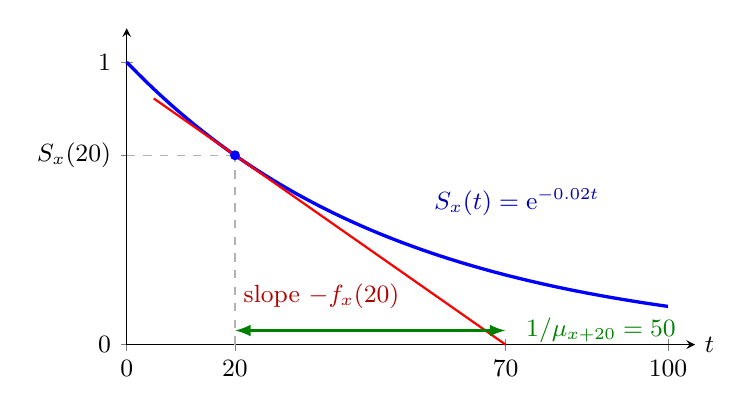
\begin{tikzpicture}[font=\small, >={Latex[length=2mm]}]
  \begin{axis}[
    axis lines=left, xmin=0, xmax=105, ymin=0, ymax=1.12,
    xtick={0,20,70,100}, ytick={0,0.6703,1}, yticklabels={$0$,$S_x(20)$,$1$},
    xlabel={$t$},
    xlabel style={at={(axis description cs:1,0)}, anchor=west},
    samples=100, width=8.8cm, height=5.6cm, clip=false]
    \addplot[blue, very thick, domain=0:100] {exp(-0.02*x)};
    \draw[gray!60, thin, dashed] (axis cs:0,0.6703) -- (axis cs:20,0.6703);
    \draw[gray!60, thin, dashed] (axis cs:20,0) -- (axis cs:20,0.6703);
    \draw[red, thick] (axis cs:5,0.8714) -- (axis cs:70,0);
    \fill[blue] (axis cs:20,0.6703) circle (1.8pt);
    \draw[<->, green!50!black, thick] (axis cs:20,0.05) -- (axis cs:70,0.05);
    \node[green!50!black, anchor=west] at (axis cs:72,0.05) {$1/\mu_{x+20}=50$};
    \node[red!70!black] at (axis cs:36,0.17) {slope $-f_x(20)$};
    \node[blue!70!black, anchor=south west] at (axis cs:55,0.42) {$S_x(t)=\mathrm{e}^{-0.02t}$};
  \end{axis}
\end{tikzpicture}
\end{document}
